\documentclass{article}
\usepackage[ruled,vlined,linesnumbered]{algorithm2e}
\usepackage{algpseudocode}
\usepackage{amsmath}
\usepackage{amsthm}
\usepackage{graphicx}
\usepackage{subfigure}
\usepackage{float}
\usepackage{amsmath }
\usepackage{amsfonts }
\usepackage{pdfpages}
\usepackage{epsfig}
\usepackage{graphicx}
\usepackage{arydshln}
\usepackage{verbatim}
\usepackage{subfigure}
\usepackage{enumerate}
\usepackage{rotating}
\usepackage{threeparttable}
\usepackage{caption}
\usepackage{epsfig}
\usepackage{cite}
\usepackage{tikz}
\usetikzlibrary{shapes}
\usetikzlibrary{shapes.geometric}
\usepackage{geometry}
\geometry{a4paper, top=2.54cm, bottom=2.54cm, left=3.18cm, right=3.18cm}
\theoremstyle{definition}
\newtheorem{prob}{Problem}
\newtheorem{ans}{Answer}
\usepackage[colorlinks,linkcolor=black]{hyperref}
\linespread{1.2}
\begin{document}
	\title{Assignment 4}
	\author{Kailing Wang 521030910356}
	\date{November 28.2022}
	\maketitle
	\begin{prob}
		(20 points) Usually, we want to improve the time complexity. But now, let us talk about space complexity.
		\begin{enumerate}[(a)]
			\item (10 points) Recall the knapsack DP algorithm in the lecture, which has $n W$ subproblems totally. We need to maintain a subproblem table with size $n \times W$. Can we use only $O(W)$ space (i.e., maintain only a $1 \times W$ size subproblem table) to implement the DP algorithm (still runs in $O(n W))$ ?
			\item (10 points) Recall the Edit Distance DP algorithm in the lecture, which has $\mathrm{nm}$ subproblems totally. Can we use only $O(\min \{n, m\})$ space to implement the DP algorithm (still runs in $O(n m))$ ?
		\end{enumerate}
	\end{prob}
	
	\begin{ans}
		~
		
		\begin{enumerate}[(a)]
			\item Suppose there are $n$ objects, and we have $W$ total capacity. The DP function is 
		
			$$
			f[i, v]=\max \{f[i-1, v], f[i-1, v-w[i]]\}
			$$
			
			In the DP we talked in class, we used a full table with $O(nW)$ space to store every subproblem. However, most of the information in the table is useless. When calculating the $k+1$th row, only the $k$th row is used. In fact, only two rows of the table is useful. Each time use one of the rows as the $k$th row and the other as the $k+1$th row. The actual space complexity is $O(n)$. If we update from right to left, only $n$ space is needed, which I find in PPT. That might be the intended solution.
			\item First review the DP edit distance. For two strings a and b with length m and n. The DP function is 
			
			$$
			d[i][j]=
			\begin{cases}
				d[i-1][j-1] & ,a[i]==b[j]\\
				\min\{d[i-1][j], d[i][j-1], d[i-1][j-1]\}+1 & ,a[i]!=b[j]
			\end{cases}
			$$
			
			Similar to the first problem, only the last one row is useful. Suppose $m<n$, we only need $2\cdot m$ space $d[2][m]$. Initialize the first column and row, and for n times do:
			
			In the $k-1$th loop, one line is initialized or calculated. In the $k$th loop, update from left to right using only the information from the last row and the left part. 
			
			The space complexity is $O(m)$. If $n<m$, transpose the process and the space complexity can be $O(n)$. The total time complexity is $O(\min\{m, n\})$.
			
			We can also do it more dynamically, and can reach $\Theta(n)$. But that will sacrifice time moving data in the memory.
		\end{enumerate}
	\end{ans}
	
	\begin{prob}
		(25 points) Given a sequence of integers $a_{1}, a_{2}, \ldots, a_{n}$, a lower bound and an upper bound $1 \leq L \leq R \leq n$. An $(L, R)$-step subsequence is a subsequence $a_{i_{1}}, a_{i_{2}}, \ldots, a_{i_{\ell}}$, such that $\forall 1 \leq j \leq \ell-1, L \leq i_{j+1}-i_{j} \leq R$. The revenue of the subsequence is $\sum_{j=1}^{\ell} a_{i_{j}}$. Design a DP algorithm to output the maximum revenue we can get from a $(L, R)$-step subsequence.
		\begin{enumerate}[(a)]
			\item (5 points) Suppose $L=R=1$. Design a DP algorithm in $O(n)$ to find the maximum $(1,1)$-step subsequence.
			\item (10 points) Design a DP algorithm in $O\left(n^{2}\right)$ to find the maximum $(L, R)$-step subsequence for any $L$ and $R$.
			\item (10 points) Design a DP algorithm in $O(n)$ to find the maximum $(L, R)$-step subsequence for any $L$ and $R$.
		\end{enumerate}
	\end{prob}
	
	\begin{ans}
		~
		
		\begin{enumerate}[(a)]
			\item The subsequence is continuous if $L=R=1$. The max revenue of the k-front sequence ($a_{1}, a_{2}, \ldots, a_{k}, k\leq n$) is only based on the (k-1)-front sequence. This is:
			
			$$
			R[k]=
			\begin{cases}
				R[k-1] &, a_k\leq0\\
				R[k-1]+a_k &, a_k>0
			\end{cases}
			$$
			
			Initialize R[0]=0, and then we can simply DP from the front to the end and select the largest $R[k]$. Correctness: for this problem, the answer is obviously the sum of all the positive numbers, and this DP can obviously achieve this. 
			\item For this condition, the $a_k$ can inherit the revenue of front sequences that end from $a_{k-R}$ to $a_{k-L}$. The $O(n^2)$ DP is to DP like the previous problem but each update takes $R-L$ time. The runtime is $O(n(R-L))=O(n^2)$. The DP function is like:
			
			$$
			R[k]=\underset{L\leq m \leq R}{\max}R[k-m]+\max\{a_k, 0\}
			$$
			
			Select the largest $R[k]$. The correctness is, assume $R[1], R[2], \ldots, R[k-1]$ are optimal, $R[k]$ must be optimal because it inherits the max revenue it can. 
			
			\item The DP structure is the same as the previous problem. To make it $O(n)$. Use potential list. The correctness of the potential list is proved in class. Anyway, I decide to prove the time complexity here. The potential list is a queue with length $R-L+1$ and the update rule is:
			\begin{itemize}
				\item For the first R elements, each time pop the queue from the end until the tail is larger than the new element, and enqueue the new element. 
				\item For the other elements, each time in addition pop the head if the head is R+1 distance away. 
			\end{itemize}
		
			This ensures the list is in descending order. And with this structure we only need $O(1)$ to select the largest legal revenue. We need $O(n)$ time complexity, and the time to maintain a potential list is the bottleneck. Consider the overall operations concerning the potential list: Every element can only enqueue once and be popped once, so the total time complexity caused by the potential list is also $O(n)$. The total is $O(n)$.
		\end{enumerate}
	\end{ans}
	
	\begin{prob}
		(25 points) Optimal Indexing for A Dictionary Consider a dictionary with $n$ different words $a_{1}, a_{2}, \ldots, a_{n}$ sorted by the alphabetical order. We have already known the number of search times of each word $a_{i}$, which is represented by $w_{i}$. Suppose that the dictionary stores all words in a binary search tree $T$, i.e., each node's word is alphabetically larger than the words stored in its left subtree and smaller than the words stored in its right subtree. Then, to look up a word in the dictionary, we have to do $\ell_{i}(T)$ comparisons on the binary search tree, where $\ell_{i}(T)$ is exactly the level of the node that stores $a_{i}$ (root has level 1). We evaluate the search tree by the total number of comparisons for searching the $n$ words, i.e., $\sum_{i=1}^{n} w_{i} \ell_{i}(T)$. Design a DP algorithm to find the best binary search tree for the $n$ words to minimize the total number of comparisons. 
	\end{prob}	
	
	\begin{ans}
		~
		
		I don't understand the trick of using words instead of simple number——it's the same problem. Consider how an optimal tree is constructed. Suppose there is an optimal tree. The left and right subtree are also optimal trees. Otherwise changing the subtrees into optimal tree the total comparison time will reduce. Therefore any subtree in the main tree is an optimal tree.
		
		First sort the words. This way, the optimal tree is constructed by selecting a root word $w_k$ each time and go on dp the left and right subtree. The words on the left of $w_k$ is on the left subtree and the other on the right.
		
		\begin{center}
		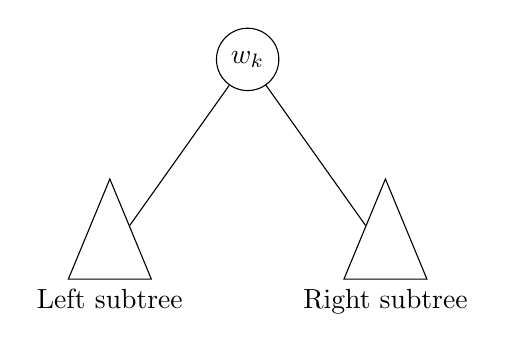
\begin{tikzpicture}[sibling distance=3.5cm,level distance=1.5cm]
			\node [draw, circle] (root) {$w_k$}
			child {node[draw, isosceles triangle, rotate=90, minimum size=30pt, anchor=apex, label=left:Left subtree] {}}
			child {node[draw, isosceles triangle, rotate=90, minimum size=30pt, anchor=apex, label=left:Right subtree,] {}};
		\end{tikzpicture}
	
		(Spent hours to learn TIKZ but failed. Want tutorial)
		\end{center}
		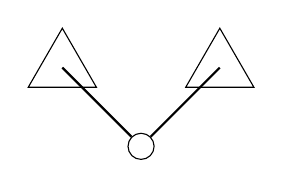
\begin{tikzpicture}
			
			% 引入 calc 包
			\usetikzlibrary{calc}
			
			% 绘制根节点
			\node[draw=black,circle,minimum size=2mm] (root) at (0,0) {};
			
			% 计算三角形的顶点坐标
			\coordinate (A) at ($(root) + (-1,1)$);
			\coordinate (B) at ($(root) + (1,1)$);
			
			% 放置三角形
			\node[draw=black,regular polygon, regular polygon sides=3, minimum size=1cm] at (A) {};
			\node[draw=black,regular polygon, regular polygon sides=3, minimum size=1cm] at (B) {};
			
			% 绘制连接线
			\draw[thick,black] (root) -- (A);
			\draw[thick,black] (root) -- (B);
			
		\end{tikzpicture}
		
		Now consider how to find the $w_k$ on a range $[i,j]\in [1,n]$. The DP function is
		
		$$
		C[i,j]=\underset{i\leq k \leq j}{\min}\{C[i, k-1]+c[k+1, j]\}+\overunderset{j}{n=i}{\Sigma}w_i
		$$
		
		Here since all the words in the subtree become 1 level deeper in the new tree, we need to add all the search time once. The naive way is to calculate all the subtrees.
		
		\begin{itemize}
			\item First initialize $C[i, i]=w_i:~O(n)$
			\item Calculate all the subtree $C[i, i+1]$ with length 2 using the DP function: $O(n-1)$
			\item Calculate all the subtree $C[i, i+2]$ with length 3: $O((n-2)*2)$
			\item Repeat, and calculate subtree $C[i, i+k]$ is $O((n-k)*k))$
		\end{itemize} 
		
		The process can also be described in a table where we initialize the diagonal and DP towards the Upper-Right corner. The total time complexity is
		 
		$$
		\begin{aligned}
			  & O(n)+\overunderset{n-1}{k=1}{\Sigma}O((n-k)*k))\\
			= & O\left(n+\frac{n(n-1)}{2}-\frac{(n-1)(n-2)(2n-3)}{6}\right)\\
			= & O(n^3)
		\end{aligned}
		$$
		
		Sadly the time complexity is not that good.
		
		The 1-length subtrees are obviously optimal. If the (k-1)-length subtrees are optimal. The DP function must get the optimal because it includes all the cases that the two subtrees are optimal, which is required by the optimal main tree. So the final tree must be optimal according tp induction.
	\end{ans}
	\begin{prob} 
		(30 points) Collecting Gift On a Grid Given $n$ gifts located on a $(m \times m)$ grid. The $i$-th gift is located at some point $\left(x_{i}, y_{i}\right)$ (integers chosen in $1 \cdots m$ ) on the grid. A player at $(1,1)$ is going to collect gifts by several Upper-Right Move. In particular, assuming the player is currently located at $(x, y)$, he can make one Upper-Right Move to another point $\left(x^{\prime}, y^{\prime}\right)$ where $x^{\prime} \geq x$ and $y^{\prime} \geq y$. The cost of this movement is $\left(x^{\prime}-x\right)^{2}+\left(y^{\prime}-y\right)^{2}$. The player will collect the $i$-th gift when he is at point $\left(x_{i}, y_{i}\right)$. There is no restriction for the number of Upper-Right Move and the final location of the player.
		\begin{enumerate}[(a)]
			\item (15 points) Design an $O\left(m^{2}\right)$ algorithm to maximize the player's profit, i.e., the sum of value he collects minus the sum of cost he pays for his Upper-Right Move.
			\item (15 points) Sometimes, $n$ can be much smaller than $m$. Can you design another algorithm that runs in $O\left(n^{2}\right)$ for this situation?
			\item (0 Points. It is for fun, you can discuss your idea with me.) Is there any difference if the player can only make Upper-Right Move among gifts? Can we still design efficient algorithm runs in $O\left(n^{2}\right), O(n m)$, and $O\left(m^{2}\right)$ ?
		\end{enumerate}
	\end{prob}
	
	\begin{ans}
		~
		
		\begin{enumerate}[(a)]
			\item The movement cost $\left(x^{\prime}-x\right)^{2}+\left(y^{\prime}-y\right)^{2}$ means any movement can be decomposed into x and y directions. However, since $x^2\geq x$, we achieve the smallest cost when going step by step. 
			
			Now consider the grid. To any place we should walk step by step or it cost us more. This means and point is reached by the point under or left to it. View the value of gift is 0 if there is not a gift. The DP function is
			
			$$
			P[i,j]=\max\{P[i-1, j], P[i,j-1]\}-1+v[i,j]
			$$ 
			
			Here the -1 means the step cost us 1 and v[i,j] is 0 or the value of the gift.
			
			We update the table either row by row or col by col until the grid is full. This DP process include all the possible route so the correctness is obvious. Since each update is $O(1)$, the time complexity equals the number of points $O(m^2)$.
			
			\item When there is not so many gift, many step in the m*m only adds the cost by one and can be replaced with a single step. Now we only care about the relative positions of the gift. Sort the gift positions twice by x and y respectively. The the sorted index is their position in the n*n grid, and we add the 0-th row and col and put (1,1) with value 0 on the position (0,0). For example, the gift on the point (114,514) have the 19th largest x and 81 largest y. So it should be on the (19,81) point on the new grid. No two gift are on the same row or col: each row or each col has one and only gift. The distance of the two rows i and j is calculated as $|y_i-y_j|$, the difference of y of the two gift on the rows. The distance between cols is calculated by the difference of x. 
			
			Now the problem is rather the same as the previous one. 
			
			$$
			P[i,j]=\max\{P[i-1, j]-d_{row}[i-1], P[i,j-1]-d_{col}[j-1]\}+v[i,j]
			$$ 
			
			The correctness and time complexity is also the same. Since now we have a n*n grid and we use $O(n\log n)$ to sort and $O(n)$ to initialize the new grid, the total time complexity is $O(n)$.
		\end{enumerate}
	\end{ans}
	
	\begin{prob}
		How long does it take you to finish the assignment (including thinking and discussing)? Give a score $(1,2,3,4,5)$ to the difficulty. Do you have any collaborators? Write down their names here.
	\end{prob}

	\begin{ans}
		~
		
		Today(28. Nov, at around 8 p.m.) I saw Professor Yuhao and his fellows(?) in GIMLID (The 5th restaurant building, SJTU). The sandwich there worth 4 score.
		
		Bujiazi. After viewing his previous assignment and his handwriting, I found myself lack the ability of English and making clear explanation. 
	\end{ans}
\end{document}